% Template source: University of Florida Department of Physics, https://www.phys.ufl.edu/courses/phy4803L/sample-paper.zip

\documentclass[aps,twocolumn,secnumarabic,nobalancelastpage,amsmath,amssymb,nofootinbib,floatfix,letterpaper]{revtex4}

% Documentclass Options
    % aps, prl, rmp stand for American Physical Society, Physical Review Letters, and Reviews of Modern Physics, respectively
    % twocolumn permits two columns, of course
    % nobalancelastpage doesn't attempt to equalize the lengths of the two columns on the last page
        % as might be desired in a journal where articles follow one another closely
    % amsmath and amssymb are necessary for the subequations environment among others
    % secnumarabic identifies sections by number to aid electronic review and commentary.
    % nofootinbib forces footnotes to occur on the page where they are first referenced
        % and not in the bibliography
    % REVTeX 4 is a set of macro packages designed to be used with LaTeX 2e.
        % REVTeX is well-suited for preparing manuscripts for submission to APS journals.


\usepackage{chapterbib}    % allows a bibliography for each chapter (each labguide has it's own)
\usepackage{color}         % produces boxes or entire pages with colored backgrounds
\usepackage{graphics}      % standard graphics specifications
\usepackage[pdftex]{graphicx}      % alternative graphics specifications
\usepackage{epsf}          % old package handles encapsulated post script issues
\usepackage{bm}            % special 'bold-math' package
\usepackage{verbatim}			% for comment environment
\usepackage[colorlinks=true]{hyperref}  % this package should be added after all others
                                        % use as follows: \url{https://urldefense.proofpoint.com/v2/url?u=http-3A__web.mit.edu_8.13&d=DwICAg&c=sJ6xIWYx-zLMB3EPkvcnVg&r=D88uS55Tats-jlFQAC1XryFUYq8B7Lk3StFbXzgsiB4&m=Vjrc9Wj5n5rkIDMPJ5VsRj2GyXC3yXmN_zDHey6dVio&s=_byqsJfgO464rVIugNWFPmbBeIYfNiJcGS1fgIwc0m4&e= }

\usepackage{subcaption}
\usepackage{float}
\usepackage{siunitx}
\usepackage{textcomp}
\usepackage{gensymb}
\usepackage{tikz}
\usepackage{multirow}
\usepackage{xcolor}

% Graph stuff
\usepackage[utf8]{inputenc}
\usepackage{pgfplots}
\usepgfplotslibrary{groupplots,dateplot}
\usetikzlibrary{patterns,shapes.arrows}
\pgfplotsset{compat=newest}
\usepackage{shellesc}
\usetikzlibrary{external}
\tikzexternalize

% Define colours
\definecolor{darkgreen}{HTML}{228833}

\usepackage[english]{babel}
\usepackage[autostyle, english=american]{csquotes}
\MakeOuterQuote{"}


\begin{document}
\title{Title here}
\author{Tyler Tian}
\noaffiliation
\date{\today}


\begin{abstract}
TODO
\end{abstract}

\maketitle

%%%%%%%%%%%%%%%%%%%%%%%%%%%%%%%%%%%%%%%%%%%%%%%%%%%%%%%%%%%%%%%%%%

\section{Introduction}

\begin{equation}
    \theta(t) = \theta_0 e^{-\frac{t}{\tau}}\cos\left(2\pi\frac{t}{T} + \phi_0\right)
    \label{eqn:model}
\end{equation}

\begin{equation}
    Q = \pi\frac{\tau}{T}
    \label{eqn:qfactor}
\end{equation}

%%%%%%%%%%%%%%%%%%%%%%%%%%%%%%%%%%%%%%%%%%%%%%%%%%%%%%%%%%%%%%%%%%

\section{Method}

\subsection{Pendulum Construction}

\begin{figure}[htb]
    \includegraphics[width=0.6\linewidth]{swingy.jpg}
    \caption{Swingy the pendulum.}
    \label{fig:swingy}
\end{figure}

The main support structure of the pendulum consists of two pieces of wood attached with screws.
This was chosen because the material was readily available, and could be substituted for any material of
similar size and suitable strength.

The pendulum uses a thin, braided string, specifically chosen to minimize twisting in order to prevent the bob from
spinning. The string is lightly wound around a nail, and then directed through a hole in the support board and held
in place by a binder clip. A flat measuring tape is secured parallel to the string to measure the string length. A
piece of green masking tape is put over the pivot nail to enable computer-vision based tracking.

The string is attached to a bob consisting of a small, red plastic cup, specifically chosen for its high colour contrast
against the background to enable precise vision tracking. The cup is loaded with coins to vary its weight since coins
have known masses.

\subsection{Pendulum Tracking}
\label{sec:tracking}

\begin{figure}[htb]
    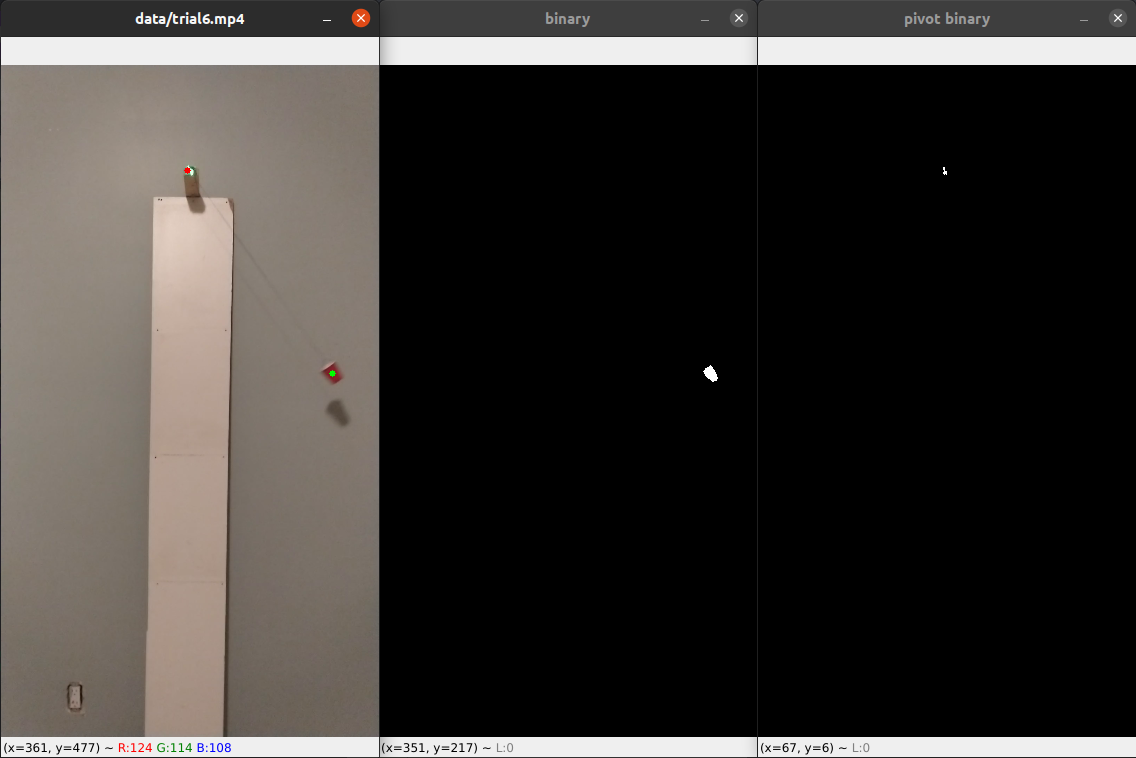
\includegraphics[width=\linewidth]{cv_track.png}
    \caption{CV-based tracking of the pendulum.}
    \label{fig:tracking}
\end{figure}

Videos of the pendulum are shot on a phone camera and then passed to a Python program written with OpenCV (see Appendix
\ref{appendix:code}). The locations of the bob and pivot are determined by thresholding the image in the HSV colour
space (the right two windows in Figure \ref{fig:tracking}), and then taking the average of the pixels that passed the
threshold to obtain the centres of the bob and pivot in the image (green and red dots in the first window in Figure
\ref{fig:tracking}). After the pixel coordinates have been determined, the ratio of the difference between the \(x\) and
\(y\) coordinates are used to compute the angle for each frame.

\subsection{Lab 1: \texorpdfstring{\(Q\)}{Q} Factor}
\label{sec:lab1_method}

For this lab, the video is shot at 60fps but only sampled at 30Hz since precise measurements are less important for
determining the \(Q\) factor. Subsequent experiments have improved this.

The string length is fixed at approximately 65cm and the mass at approximately 42g. The precise masses and lengths are
never measured as they remained constant and are unimportant for this lab.

The \(Q\) factor is obtained from the angle-time data using two independent methods:
\begin{enumerate}
    \item
        \textbf{Curve fitting:} A Python program (see Appendix \ref{appendix:code}) is used to fit the model (Equation
        \ref{eqn:model}) to the data, producing values for \(\tau\) and \(T\). \(Q\) is calculated from these values
        using Equation \ref{eqn:qfactor}.
    \item
        \textbf{Oscillation counting:} By substituting \(t = T\frac{Q}{n}\) (i.e. \(\frac{Q}{n}\) oscillations) into
        the decay term in Equation \ref{eqn:model}, the term becomes
        \begin{equation}
            \theta_0 e^{-\frac{T\frac{Q}{n}}{\tau}} = \theta_0 e^{-\frac{T\frac{\pi\frac{\tau}{T}}{n}}{\tau}} = \theta_0 e^{-\frac{\pi}{n}}
        \end{equation}
        which shows that \(\frac{Q}{n}\) can be measured by counting the number of oscillations of the pendulum until
        its amplitude decays to a factor of \(e^{-\frac{\pi}{n}}\) times the initial amplitude at release.
        
        A Python program (see Appendix \ref{appendix:code}) is used to count these oscillations. Half-oscillations are
        counted as the pendulum swings from a positive peak to a negative peak. For example, if the pendulum starts on
        the right, but first reaches the target amplitude when it is swinging to the left, then a half-oscillation will
        be counted for the last cycle. \(\frac{Q}{3}\) is measured for this lab because not enough oscillations were
        recorded to measure for \(\frac{Q}{2}\) or \(Q\) directly.
\end{enumerate}

\subsection{Lab 2: Relationship Between Period and Amplitude}
\label{sec:lab2_method}

For this lab, the video is shot at 120fps to reduce motion blur caused by the increased speeds of the bob, but the video
is still sampled at 30Hz. The string length and bob mass are the same as Lab 1 (Section \ref{sec:lab1_method}).

To convert from raw time-angle data to amplitude-period data required for this lab, a Python program was used to find
the peaks and valleys of the graph, as shown in Figure \ref{fig:rawdata} (see Appendix \ref{appendix:code}).
Since the data was somewhat noisy, multiple peak points were averaged to find the time of each peak, and the
maximum/minimum of these peak points were taken to find the peak amplitude.

\begin{figure}[htb]
    \begin{tikzpicture}
        \begin{axis}[
            title=Angle vs. Time,
            xlabel=Time (s),
            ylabel=Angle (rad),
            legend entries={Raw Data, Min/Max}
        ]
            \addplot+[
                only marks,
                mark size=1pt,
            ] table [x index=0, y index=1] {trial1_rawdata.txt};
            \addplot+[
                only marks,
                mark size=1.5pt,
            ] table [x index=0, y index=1] {trial1_extrema.txt};
        \end{axis}
    \end{tikzpicture}
    \caption{Zoomed-in view of the first 500 raw data points with the peaks marked.}
    \label{fig:rawdata}
\end{figure}

Measuring the period by taking the time for multiple oscillations and dividing by the number of oscillations will reduce
the period uncertainty, but increase the amplitude uncertainty as the amplitude decays more over a longer period of
time. Conversely, taking the time for half an oscillation and then multiplying by 2 increases the period uncertainty but
reduces the amplitude uncertainty as there is now less decay. Because the \(Q\) factor as determined in Lab 1 (Section
\ref{sec:lab1_analysis}) is reasonably but not extremely large, the period is measured directly using the difference in
time between adjacent peaks, without averaging over multiple oscillations or looking at half an oscillation.

\subsection{Lab 3: Relationship Between Period and Length/Mass}

For this lab, the video was shot at 30fps and sampled at 30Hz. As determined in Lab 2 (Section \ref{sec:lab2_analysis}),
the does have an impact on period, but this effect can be ignored for sufficiently small angles. Therefore the release
angle of the pendulum in this lab is always less than the constraint determined in Section \ref{sec:lab2_validrange}.
As the effect of decaying period is now negligible, multiple (about 10 each) oscillations were measured for every
length/mass.

The period produced by each length/mass is determined using the same method as outlined in Section
\ref{sec:lab2_method}, with yet another Python program (see Appendix \ref{appendix:code}).

To determine the effective string length, the bob is raised to the top as shown in Figure \ref{fig:raised_bob}, and a
reading is taken on the measuring tape shown in the left of Figure \ref{fig:swingy} and used as a base value. For
every trial, a reading is taken and subtracted from this base value to determine the added length.

\begin{figure}[htb]
    \includegraphics[width=0.7\linewidth]{bob_top.jpg}
    \caption{Reducing the string length to the shortest possible.}
    \label{fig:raised_bob}
\end{figure}

To determine the remaining length between the pivot and the bob's centre of mass in Figure \ref{fig:raised_bob}, a
measuring tape is used. Since the cup is much lighter than the coins inside, the centre of mass is estimated to be the
centre of mass of the 6 coins inside. The distance between the top of the 3rd coin and the pivot is measured and added
to each length to determine the final effective length.

To determine the bob's mass, the cup's mass is measured on a digital scale. Due to the activity being completed at home,
high-precision scales are often unavailable, so the mass of the coins inside is calculated using masses found on the
\href{https://www.mint.ca/store/mint/learn/canadian-circulation-1100028}{Royal Canadian Mint website}.

%%%%%%%%%%%%%%%%%%%%%%%%%%%%%%%%%%%%%%%%%%%%%%%%%%%%%%%%%%%%%%%%%%

\section{Lab 1 Results and Analysis}

\subsection{Uncertainties}
\label{sec:lab1_uncert}

There are two sources of measurement uncertainty during the data collection process shared by both methods:
\begin{enumerate}
    \item 
        \textbf{Time measurement uncertainty from the camera's frame rate and shutter speed.} Because the camera only
        captures a set number of frames per second, this creates a small uncertainty about the exact time that data
        points occurred. An upper bound for this uncertainty can be obtained by taking the time between two frames and
        dividing by 2. For a 60fps video, this results in an uncertainty of \(\pm 0.008\si{s}\).
    \item
        \textbf{Angle measurement uncertainty from motion blur and imperfect tracking.} Motion blur caused by a
        fast-moving bob can make the angle hard to measure, and imperfect computer vision tracking of the bob and
        pivot may also result in an incorrect angle. To estimate an upper bound of this uncertainty, a frame is taken
        from when the pendulum has its maximum velocity to maximize motion blur. Two lines are drawn representing the
        worst possible cases for tracking (Figure \ref{fig:angle_uncert}), and the angle between them is taken. The
        result is a range of about \(5\degree\), or an uncertainty of \(\pm 3\degree\)/\(\pm 0.05\si{rad}\).
        
        (Note: Further analysis of the behaviour of the tracking program shows this to be an overly conservative
        estimate, since the averaging of the pixel coordinates as described in Section \ref{sec:tracking} produces the
        centre of the bob reliably even when there is motion blur. Thus, while this uncertainty is shown in the later
        graphs, it is not used in the final analysis.)
\end{enumerate}
\begin{figure}[htb]
    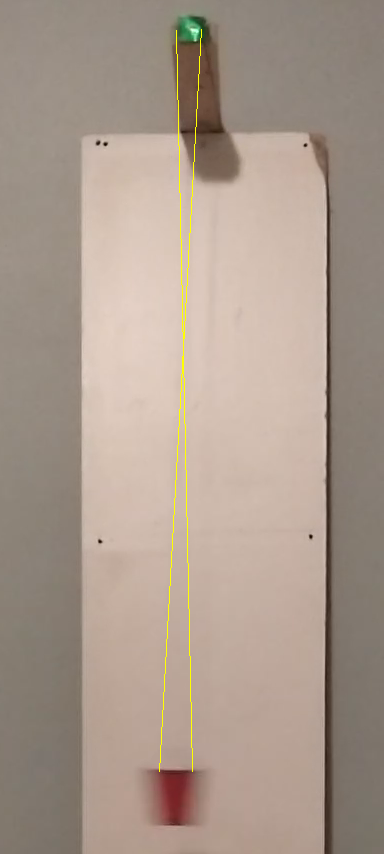
\includegraphics[width=0.3\linewidth]{uncert1.png}
    \caption{Worst-case scenarios for angle uncertainty. Blue lines are drawn to indicate the greatest and least
        possible angle. Note that this is a very conservative estimate.}
    \label{fig:angle_uncert}
\end{figure}

These uncertainties are shown in the graphs in Figure \ref{fig:lab1_fitzoom}. They are very small when
compared to the uncertainties later in the experiment, and so they will be ignored as only the largest uncertainty is
considered for this lab.

There are also other sources of measurement uncertainty that are much harder to quantify, such as perspective
distortion and camera tilt. These uncertainties are assumed to be smaller and random, and thus incorporated in other
sources.

Specifically for method 1 (curve fitting), the least-squares fit generates a covariance matrix, which contains the
standard deviations of each fit parameters. These standard deviations are used as the uncertainties for \(\tau\) and
\(T\), and propagated to \(Q\) by taking the largest relative uncertainty.

Specifically for method 2 (oscillation counting), amplitude can only be determined at a positive or negative peak, which
gives the oscillation count a maximum resolution of 0.5 (Section \ref{sec:lab1_method}). When multiplied by 3 to find
\(Q\), this represents an uncertainty of \(\pm 1.5\).

For both methods, 7 trials were conducted, and the uncertainty of the mean of these trials is used as another source of
uncertainty.

\subsection{Results from Curve Fitting}

\begin{figure*}[t]
    \centering
    \begin{subfigure}{\textwidth}
        \begin{tikzpicture}
            \begin{axis} [
                title=Best Fit Curve,
                xlabel=Time (s),
                ylabel=Angle (rad),
                width=\textwidth,
                height=0.2\textheight,
                xmin=-3,
                xmax=120,
                extra y ticks={0},
                extra y tick labels={},
                extra y tick style={grid=major},
                clip marker paths=true,
                legend entries={Collected Data, Best Fit Curve}
            ]
                \addplot+[
                    only marks,
                    mark size=1pt,
                ] table [
                    x index=0,
                    y index=1,
                ] {lab1_data.txt};
                \addplot [
                    thick,
                    red,
                    domain=0:117,
                    samples=2000,
                ] {0.6057992432358721 * e ^ (-x / 80.4722570265344) * cos(deg(2 * pi * x / 1.6499108861456369 - 0.6356025015941729))};
            \end{axis}
        \end{tikzpicture}
        \begin{tikzpicture}
            \begin{axis} [
                title=Fit Residuals,
                xlabel=Time (s),
                ylabel=Angle (rad),
                width=\textwidth,
                height=0.2\textheight,
                xmin=-3,
                xmax=120,
                extra y ticks={0},
                extra y tick labels={},
                extra y tick style={grid=major},
            ]
                \addplot+[
                    only marks,
                    mark size=1pt
                ] table [
                    x index=0,
                    y index=2,
                ] {lab1_data.txt};
            \end{axis}
        \end{tikzpicture}
        \caption{Result of fitting Equation \ref{eqn:model} to one of the trials. For this particular fit, \(A = 0.606\),
            \(\tau = 80.5\), \(T = 1.65\), \(\phi = -0.636\). Uncertainty bars are omitted to improve readability.}
        \label{fig:lab1_fit}
    \end{subfigure}
    \begin{subfigure}{\textwidth}
        \begin{tikzpicture}
            \begin{axis} [
                title=Best Fit Curve,
                xlabel=Time (s),
                ylabel=Angle (rad),
                width=\textwidth,
                height=0.2\textheight,
                xmin=-0.5,
                xmax=10.5,
                extra y ticks={0},
                extra y tick labels={},
                extra y tick style={grid=major},
                clip marker paths=true,
                legend entries={Collected Data, Best Fit Curve}
            ]
                \addplot+[
                    only marks,
                    mark size=1pt,
                    restrict expr to domain={x}{0:10},
                    error bars/.cd,
                        x dir=both,
                        y dir=both,
                        x explicit,
                        y explicit,
                        x fixed=0.008,
                        y fixed=0.05,
                ] table [
                    x index=0,
                    y index=1,
                ] {lab1_data.txt};
                \addplot [
                    thick,
                    red,
                    domain=0:10,
                    samples=200,
                ] {0.6057992432358721 * e ^ (-x / 80.4722570265344) * cos(deg(2 * pi * x / 1.6499108861456369 - 0.6356025015941729))};
            \end{axis}
        \end{tikzpicture}
        \begin{tikzpicture}
            \begin{axis} [
                title=Fit Residuals,
                xlabel=Time (s),
                ylabel=Angle (rad),
                width=\textwidth,
                height=0.2\textheight,
                xmin=-0.5,
                xmax=10.5,
                extra y ticks={0},
                extra y tick labels={},
                extra y tick style={grid=major},
            ]
                \addplot+[
                    only marks,
                    mark size=1pt,
                    restrict expr to domain={x}{0:10},
                    error bars/.cd,
                        x dir=both,
                        y dir=both,
                        x explicit,
                        y explicit,
                        x fixed=0.008,
                        y fixed=0.05,
                ] table [
                    x index=0,
                    y index=2,
                ] {lab1_data.txt};
            \end{axis}
        \end{tikzpicture}
        \caption{Zoomed-in view of the first 15 seconds of the data, showing the uncertainties. Note the significant
            deviation of the best-fit curve from the actual data.}
        \label{fig:lab1_fitzoom}
    \end{subfigure}
    \caption{Fitting Equation \ref{eqn:model} to data from one of the trials.}
    \label{fig:lab1_graph}
\end{figure*}

Figure \ref{fig:lab1_graph} shows the result of fitting Equation \ref{eqn:model} for one of the trials.
\(Q\) values computed using this method are shown in Table \ref{table:lab1_fit}.

\begin{table}[h]
    \begin{tabular}{c|c|c|c}
        Trial & \(Q\) & Uncertainty & \% Uncertainty \\
        \hline
        1   & 153.23    & \(\pm 3.65\) & 2.38 \\
        2   & 147.89    & \(\pm 3.95\) & 2.67 \\
        3	& 140.96	& \(\pm 3.53\) & 2.51 \\
        4	& 151.12	& \(\pm 3.81\) & 2.52 \\
        5	& 130.24	& \(\pm 3.86\) & 2.96 \\
        6	& 131.31	& \(\pm 3.76\) & 2.86 \\
        7	& 138.04	& \(\pm 3.70\) & 2.68 \\
        \hline
        \multicolumn{3}{l}{Mean} & 141.83 \\
        \multicolumn{3}{l}{Standard Deviation} & 9.24 \\
        \multicolumn{3}{l}{Uncertainty of the Mean} & 3.49
    \end{tabular}
    \caption{Raw data from curve fitting; values are unrounded.}
    \label{table:lab1_fit}
\end{table}

From Table \ref{table:lab1_fit}, the greatest percentage uncertainty is trial 5 with an uncertainty of 2.96\%. When
multiplied by the mean, this corresponds to an uncertainty of \(\pm 4.20\), which is greater than the uncertainty of
the mean. \textbf{The final value as determined by this method is \(Q = 142 \pm 4\).}

\subsection{Results from Oscillation Counting}

\(Q\) values computed using this method are shown in Table \ref{table:lab1_osc}.

\begin{table}[h]
    \begin{tabular}{c|c|c|c}
        Trial & \(Q\) & Uncertainty & \% Uncertainty \\
        \hline
        1   & 148.5 & \(\pm 1.5\) & 1.01 \\
        2   & 151.5 & \(\pm 1.5\) & 0.99 \\
        3	& 148.5 & \(\pm 1.5\) & 1.01 \\
        4	& 154.5 & \(\pm 1.5\) & 0.97 \\
        5	& 139.5 & \(\pm 1.5\) & 1.08 \\
        6	& 142.5 & \(\pm 1.5\) & 1.05 \\
        7	& 148.5 & \(\pm 1.5\) & 1.01 \\
        \hline
        \multicolumn{3}{l}{Mean} & 147.6 \\
        \multicolumn{3}{l}{Standard Deviation} & 5.11 \\
        \multicolumn{3}{l}{Uncertainty of the Mean} & 1.93
    \end{tabular}
    \caption{Raw data from oscillation counting; values are unrounded.}
    \label{table:lab1_osc}
\end{table}

From Table \ref{table:lab1_osc}, the greatest percentage uncertainty is trial 5 with an uncertainty of 1.08\%, which
corresponds to an uncertainty of \(\pm 1.59\) in \(Q\), less than the uncertainty of the mean. \textbf{The final value
as determined by this method is \(Q = 148 \pm 2\).}

However, an interesting phenomenon can be observed by varying the fraction of \(Q\) to measure for.
For example, by measuring for \(\frac{Q}{4}\) instead, the data in Table \ref{table:lab1_osc4} is obtained, which has a
significantly different mean \(Q\) value.

\begin{table}[h]
    \begin{tabular}{c|c|c|c}
        Trial & \(Q\) & Uncertainty & \% Uncertainty \\
        \hline
        1   & 126.0 & \(\pm 2\) & 1.59 \\
        2   & 138.0 & \(\pm 2\) & 1.45 \\
        3	& 134.0 & \(\pm 2\) & 1.49 \\
        4	& 144.0 & \(\pm 2\) & 1.39 \\
        5	& 128.0 & \(\pm 2\) & 1.56 \\
        6	& 126.0 & \(\pm 2\) & 1.59 \\
        7	& 134.0 & \(\pm 2\) & 1.49 \\
        \hline
        \multicolumn{3}{l}{Mean} & 132.9 \\
        \multicolumn{3}{l}{Standard Deviation} & 6.72 \\
        \multicolumn{3}{l}{Uncertainty of the Mean} & 2.54
    \end{tabular}
    \caption{Data obtained from measuring \(\frac{Q}{4}\) instead; values are unrounded. Note how the mean
        \(Q\) value deviates significantly from the one obtained in Table \ref{table:lab1_osc}.}
    \label{table:lab1_osc4}
\end{table}

After more trials, it was observed that the value of \(Q\) obtained through counting oscillations is dependent on the
fraction of \(Q\) that was counted for. Moreover, as the denominator increases, the observed \(Q\) value seems to
decrease. This is not in agreement with the model since according to Equations \ref{eqn:model} and \ref{eqn:qfactor}
\(Q\) should be independent of the fraction measured.

\subsection{Discussion and Analysis}
\label{sec:lab1_analysis}

\subsubsection{\texorpdfstring{\(Q\)}{Q} Factor}
\label{sec:lab1_qfactor}

The \(Q\) value obtained by oscillation counting is within 1.5 times the uncertainty of the \(Q\) value obtained by
curve fitting. If values follow a normal distribution, there is a 13.4\% chance for values to be more than 1.5 times the
uncertainty away. From this we conclude that \textbf{while there is a discrepancy between the two \(Q\) values, the
values could be in agreement.}

However, as shown in Table \ref{table:lab1_osc4}, by measuring for \(\frac{Q}{4}\) a \(Q\) value of \(133 \pm 3\) is
obtained instead. This value is 2.25 times the uncertainty away from the \(Q\) value obtained by curve fitting, and 5
times the uncertainty away from the \(Q\) value obtained by counting for \(\frac{Q}{3}\), which clearly disagrees with
either \(Q\) value found above.

Furthermore, as the fraction of \(Q\) measured for gets smaller, the measured \(Q\) value gets even further from the
values obtained previously. It can be concluded that, at least for this particular pendulum, \textbf{oscillation
counting is not a reliable way for obtaining \(Q\)}. As a result, the final \(Q\) value is taken to be the one obtained
through curve fitting (\(Q = 142 \pm 4\)).

\subsubsection{Model Accuracy}

\begin{figure*}[t]
    \begin{tikzpicture}
        \begin{axis} [
            title=Best Fit Curve,
            xlabel=Time (s),
            ylabel=Angle (rad),
            width=\textwidth,
            height=0.2\textheight,
            xmin=-3,
            xmax=120,
            extra y ticks={0},
            extra y tick labels={},
            extra y tick style={grid=major},
            clip marker paths=true,
            legend entries={Collected Data, Best Fit Curve}
        ]
            \addplot+[
                only marks,
                mark size=1pt,
            ] table [
                x index=0,
                y index=1,
            ] {lab1_data2.txt};
            \addplot [
                thick,
                red,
                domain=0:117,
                samples=2000,
            ] {0.663973140409552 * e ^ (-x / 55.2123562331802) * cos(deg(2 * pi * x / 1.656087056926946))};
        \end{axis}
    \end{tikzpicture}
    \begin{tikzpicture}
        \begin{axis} [
            title=Fit Residuals,
            xlabel=Time (s),
            ylabel=Angle (rad),
            width=\textwidth,
            height=0.2\textheight,
            xmin=-3,
            xmax=120,
            extra y ticks={0},
            extra y tick labels={},
            extra y tick style={grid=major},
        ]
            \addplot+[
                only marks,
                mark size=1pt
            ] table [
                x index=0,
                y index=2,
            ] {lab1_data2.txt};
        \end{axis}
    \end{tikzpicture}
    \caption{Result of fitting to the same data but with \(\phi_0 = 0\) (Equation \ref{eqn:model_nophi}). For this
        particular fit, \(A = 0.664\), \(\tau = 55.2\), \(T = 1.66\). Uncertainty bars are omitted to improve readability.}
    \label{fig:lab1_fit2}
\end{figure*}

An inspection of the residuals in Figure \ref{fig:lab1_graph} shows a clear pattern, which would not be present if the fit
represents the data well. At many points, the residuals reach a value of 0.2, which is over 25\% of the actual
amplitude of the data, 0.8. The amplitude of the fit also deviates significantly from the actual amplitude of the data
(0.6 versus 0.8), but adjusting the conditions of the fit does not improve it. The fit also seems to deviate
significantly from the actual data near the beginning and end of the data set as shown in Figure \ref{fig:lab1_fitzoom}.

The two possible reasons for this happening are either that the fit was not done well, or the model does not reflect the
real data well. The data is inconclusive for determining which is the dominant effect for sure, but there is evidence to
suggest that the model may not be entirely accurate.

Since time \(t = 0\) is taken to be when the pendulum is first released, the theoretical value of \(\phi_0\) should
always be 0, so the model is reduced to
\begin{equation}
    \theta(t) = \theta_0 e^{-\frac{t}{\tau}}\cos\left(2\pi\frac{t}{T}\right)
    \label{eqn:model_nophi}
\end{equation}

However, all the trials produce nonzero values for \(\phi_0\). The result of fitting to the same data but with
\(\phi_0\) removed is shown in Figure \ref{fig:lab1_fit2}. Compared to Figure \ref{fig:lab1_fit}, this time the fit is
much worse, with the fit curve deviating significantly from the data in both magnitude and phase near the end, where
visually the fit seems to be off by more than \(\frac{1}{4}\) of a period. The residuals seem to keep on increasing at
the end and are much larger than the uncertainties, which shows that \textbf{Equation \ref{eqn:model} is not an
accurate model of this pendulum for large values of \(t\)}.

This might be because Equation \ref{eqn:model} is derived with the simplifying assumption of \(\sin \theta \approx \theta\)
for small angles, which produces a restoring force that is proportional to angle. Since \(\theta > \sin \theta\) for
\(\theta \neq 0\), the restoring force predicted by the model is always larger than the real force, producing a larger
acceleration and velocity. Since the damping force due to viscous air friction is proportional to velocity, the larger
velocity predicted by the model leads to more damping and thus more decay. This is consistent with Figures
\ref{fig:lab1_fit} and \ref{fig:lab1_fit2}, both of which show that the actual rate of decay is slower than the
predicted rate of decay.

Another reason for the large residuals could be that the period of this pendulum appears to be non-constant.
Observing the data more closely shows that the period of the pendulum appears to decrease slightly as time progresses.
In particular, for the trial in Figure \ref{fig:lab1_graph}, the initial period shortly after release is about
\(1.67\si{s} \pm 0.01\si{s}\), while the final period near the end of the video is about \(1.64\si{s} \pm 0.01\si{s}\).
Although the difference is small, it is consistently present throughout multiple trials and is too large to be explained
by uncertainties. This is consistent with Figures \ref{fig:lab1_fit} and \ref{fig:lab1_fit2}, both of which show that
the period predicted by Equation \ref{eqn:model} is different from the actual period, since the fit and the actual data
become out of phase as time goes on. The relationship between period and other parameters is investigated in more
detail in the following Labs.

%%%%%%%%%%%%%%%%%%%%%%%%%%%%%%%%%%%%%%%%%%%%%%%%%%%%%%%%%%%%%%%%%%

\section{Lab 2 Results and Analysis}

\subsection{Uncertainties}

The sources of measurement uncertainty are the following:
\begin{enumerate}
    \item
        \textbf{Time (period) uncertainty from the camera/sampling speed:} A set number of data points is collected per
        second, which means the true peak of an oscillation could lie between two data points. When this happens, the
        precise location of the peak cannot be determined, creating an uncertainty. An upper bound for this uncertainty
        can be obtained by taking the time between data points dividing by 2. At 30 data points per second, this results
        in an uncertainty of \(\pm 0.02\si{s}\).
    \item
        \textbf{Period uncertainty from noise in the data and inaccuracies in peak finding:} Due to noise in the data,
        sometimes the true peak location is not apparent, with multiple locations looking like potential peaks. The code
        attempts to correct this by taking the mean of all peak candidates. The uncertainty of the mean
        (\(\frac{\sigma}{\sqrt{N}}\)) of the peak candidates is used as the uncertainty, which is computed individually
        for each data point.
    \item
        \textbf{Amplitude uncertainty caused by the previous two uncertainties:} Since the true peak may lie between two data
        points (as per \textcircled{1}) and is influenced by noise (as per \textcircled{2}), this creates an
        uncertainty regarding the amplitude of the peak. As the exact value of this uncertainty is hard to find, it is
        assumed to be the same in percentage as the larger of \textcircled{1} and \textcircled{2}.
    \item
        \textbf{Amplitude uncertainty caused by the decay of the pendulum over one oscillation:} The pendulum's
        amplitude decays as it swings, creating an uncertainty. By substituting \(t = T\) into the pendulum equation, we
        obtain an exponential term of \(e^{-\frac{T}{t}} = e^{-\frac{\pi}{Q}}\). In other words, the amplitude decays by
        a factor of \(e^{-\frac{\pi}{Q}}\) per oscillation. The relative change in amplitude is then
        \(1 - e^{-\frac{\pi}{Q}}\); by substituting in the \(Q\) value obtained in Section \ref{sec:lab1_qfactor}, the
        amount of decay is found to be \(2.19\%\), so the uncertainty is \(\pm 2\%\).
\end{enumerate}

Plotting the data points obtained from one trial with the uncertainties yields Figure \ref{fig:lab2_data1}.

\begin{figure}[htb]
    \begin{tikzpicture}
        \begin{axis}[
            title=Period vs. Amplitude,
            xlabel=Amplitude (rad),
            ylabel=Period (s),
            xmin=-2,
            xmax=2,
        ]
            \addplot+[
                only marks,
                mark size=1pt,
                error bars/.cd,
                    x dir=both,
                    y dir=both,
                    x explicit,
                    y explicit,
            ] table [
                x index=0,
                y index=1,
                x error index=2,
                y error index=3,
            ] {lab2_data1.txt};
        \end{axis}
    \end{tikzpicture}
    \caption{Data points collected from one trial, plotted with uncertainty bars.}
    \label{fig:lab2_data1}
\end{figure}

Additionally, just like in Section \ref{sec:lab1_uncert}, the least-squares fit also produces standard deviations that
can be used as uncertainties.

\subsection{Results}

Data points collected from all 5 trials are combined for the fit.
Table \ref{table:lab2_fit} shows the optimal parameters resulting from fitting power series of various degrees to the
data. Note that the parameter and uncertainty values in Table \ref{table:lab2_fit} are unrounded to allow for later
analysis; refer to later sections for properly rounded values.

The uncertainties in Table \ref{table:lab2_fit} take into account both the uncertainties of the fit and the measurement
uncertainties in the period and amplitude data that carries through, by taking the maximum of the two. The maximum
relative uncertainty for any data point was determined to be 2.95\%.

\begin{table}[h]
    \begin{tabular}{c|c|r|r}
        Degree & Param. & \multicolumn{1}{c|}{Value} & \multicolumn{1}{c}{Max Uncertainty} \\
        \hline
        0                  & $T_0$ & 1.662 & \pm 0.0490 \\
        \hline
        \multirow{2}{*}{1} & $T_0$ & 1.662 & \pm 0.0490 \\
                           & $B$ & -0.00298 & \pm 0.00283 \\
        \hline
        \multirow{3}{*}{2} & $T_0$ & 1.633 & \pm 0.0481 \\
                           & $B$ & 0.00257 & \pm 0.00129 \\
                           & $C$ & 0.1109 & \pm 0.00327 \\
        \hline
        \multirow{4}{*}{3} & $T_0$ & 1.633 & \pm 0.0481 \\
                           & $B$ & 0.00323 & \pm 0.00201 \\
                           & $C$ & 0.1108 & \pm 0.00326 \\
                           & $D$ & -0.000788 & \pm 0.00190 \\
        \hline
        \multirow{5}{*}{4} & $T_0$ & 1.634 & \pm 0.0481 \\
                           & $B$ & 0.00283 & \pm 0.00202 \\
                           & $C$ & 0.1041 & \pm 0.00449 \\
                           & $D$ & -0.000177 & \pm 0.00194 \\
                           & $E$ & 0.00431 & \pm 0.00270 \\
    \end{tabular}
    \caption{Optimal parameters from the fit for various degrees. Note the values and uncertainties are unrounded.}
    \label{table:lab2_fit}
\end{table}

Graphs of the fit and residuals are shown for degrees 0 to 2 in Figures \ref{fig:lab2_fit} to \ref{fig:lab2_residuals2}.
Uncertainty bars are omitted for Figure \ref{fig:lab2_fit} to keep the graph readable, since there are too many data
points.

\begin{figure*}[t]
    \centering
    \begin{subfigure}{\textwidth}
        \begin{tikzpicture}
            \begin{axis}[
                title=Period vs. Amplitude,
                xlabel=Amplitude (rad),
                ylabel=Period (s),
                xmin=-1.8,
                xmax=1.8,
                xtick distance=0.3,
                legend entries={Collected Data, Degree 0 Fit, Degree 1 Fit, Degree 2 Fit},
                legend style={
                    at={(0.5, 0.98)},
                    anchor=north
                },
                width=\textwidth,
                height=0.5\textwidth,
            ]
                \addplot+[
                    black,
                    mark options={fill=black},
                    only marks,
                    mark size=1pt,
                ] table [x index=0, y index=1] {lab2_fit_data.txt};
                \addplot[
                    blue,
                    very thick,
                    domain=-1.6:1.6,
                    samples=3,
                ] {1.662};
                \addplot[
                    red!75!white,
                    very thick,
                    domain=-1.6:1.6,
                    samples=3,
                ] {1.662 - 0.00298*x};
                \addplot[
                    darkgreen,
                    very thick,
                    domain=-1.6:1.6,
                    samples=200,
                ] {1.633 + 0.00257*x + 0.1109*x^2};
            \end{axis}
        \end{tikzpicture}
        \caption{Result of fitting a 0, 1, and 2 degree power series to the data. Error bars are omitted for readability.}
        \label{fig:lab2_fit}
    \end{subfigure}
    \begin{subfigure}{0.49\textwidth}
        \begin{tikzpicture}
            \begin{axis}[
                title=Residuals for Degree 0 Fit,
                xlabel=Amplitude (rad),
                ylabel=Period (s),
                extra y ticks={0},
                extra y tick labels={},
                extra y tick style={grid=major}
            ]
                \addplot+[
                    only marks,
                    mark size=1pt,
                    error bars/.cd,
                        x dir=both,
                        y dir=both,
                        x explicit,
                        y explicit,
                ] table [
                    x index=0,
                    y index=1,
                    x error index=2,
                    y error index=3,
                ] {residuals_deg0.txt};
            \end{axis}
        \end{tikzpicture}
        \caption{Residuals from fitting the data to \(T(\theta) = T_0\).}
        \label{fig:lab2_residuals0}
    \end{subfigure}
    \begin{subfigure}{0.49\textwidth}
        \begin{tikzpicture}
            \begin{axis}[
                title=Residuals for Degree 2 Fit,
                xlabel=Amplitude (rad),
                ylabel=Period (s),
                extra y ticks={0},
                extra y tick labels={},
                extra y tick style={grid=major},
                yticklabel style={
                    /pgf/number format/precision=3,
                    /pgf/number format/fixed
                }
            ]
                \addplot+[
                    only marks,
                    mark size=1pt,
                    error bars/.cd,
                        x dir=both,
                        y dir=both,
                        x explicit,
                        y explicit,
                ] table [
                    x index=0,
                    y index=1,
                    x error index=2,
                    y error index=3,
                ] {residuals_deg2.txt};
            \end{axis}
        \end{tikzpicture}
        \caption{Residuals from fitting the data to \(T(\theta) = T_0 + B\theta + C\theta^2\).}
        \label{fig:lab2_residuals2}
    \end{subfigure}
    \caption{Fitting power series of various degrees to the period-amplitude data.}
    \label{fig:lab2_graph}
\end{figure*}

\subsection{Discussion and Analysis}

\subsubsection{Asymmetry}

Asymmetry in the pendulum is indicated by a nonzero coefficient on the odd-powered terms in the series (\(B, D, \cdots\)).
This is because \((-\theta)^n = \theta^n\) for even \(n\), i.e. all the even terms behave identically regardless of the
sign of the angle. On the other hand, for odd \(n\), \((-\theta)^n = -\theta^n \neq \theta^n\), which means these terms behave
differently depending on the sign of \(\theta\). Thus a nonzero coefficient on the odd terms would indicate different
behaviour depending on the side that the bob is released on.

From Table \ref{table:lab2_fit}, for all the cases where \(B\) is a parameter, its value never exceeds more than 2 times its
uncertainty. Furthermore, for most of the fits, \(B\) is about or less than 1.5 times its uncertainty, therefore
\(B\) is consistent with zero. Additionally, for all the cases where \(D\) is a parameter, its value is always much less
than its uncertainty, so \(D\) is experimentally zero. As both odd terms are consistent with zero, it can be
concluded that \textbf{there is no asymmetry in the pendulum}.

\subsubsection{Relationship Between Period and Amplitude}

From simply observing Figure \ref{fig:lab2_fit}, it is clear that the data forms a distinct pattern that is not
well-approximated by a constant or linear model of \(T(\theta)\). Indeed, the value of \(C\), the coefficient on the
quadratic term, is always much larger than its uncertainty (always more than \(20 \times\)).

By examining the residuals of the degree 0 fit in Figure \ref{fig:lab2_residuals0}, it is clear that \(T(\theta) = T_0\)
is not a correct model for the data, as there is a clear parabolic pattern in the residuals, with some points having a
residual more than 5 times their uncertainty. On the other hand, the residuals of the degree 2 fit in Figure
\ref{fig:lab2_residuals2} exhibit no clear pattern, especially when \(\theta\) is large.

Note there appears to be a pattern resembling a downward parabola in Figure \ref{fig:lab2_residuals2} when \(\theta\) is
small. This can be attributed to the discretization of time due to the data collection method. Because angle data is
taken 30 times per second, the period has a resolution of \(1/30\si{s}\) without averaging. This is evident in Figure
\ref{fig:lab2_fit} as most data points seem to lie on discrete horizontal lines. Despite the pattern, the residual
points are evenly distributed above and below the zero line, indicating a good fit.

Furthermore, the higher-degree terms \(D\) and \(E\) are both smaller than 2 times their uncertainties, so they are
consistent with zero. This suggests that even for higher degrees of the fit, the terms with degree
higher than 2 should all be consistent with zero. Additionally, as \(B\) is shown to be consistent with zero in the
previous subsection, it can be concluded that the actual \(T(\theta)\) has a form of \(T(\theta) = T_0 + C\theta^2\),
i.e. \textbf{there exists a quadratic relationship between period and amplitude}.

Rounding the parameters and uncertainties gives the final equation
\begin{equation}
    T(\theta) = (1.63\si{s} \pm 0.05\si{s}) + (0.111\si{s} \pm 0.003\si{s})\theta^2
\end{equation}

\subsection{Valid Range of Constant Period Approximation}

Since the relationship between period and amplitude is actually quadratic in nature, the approximation that
\(T(\theta) = T_0\) (i.e. the period is constant) is only valid for small angles where \(\theta^2 \approx 0\). Since
Lab 3 assumes the period is constant with respect to amplitude, the range of angles for which this approximation is
valid must be determined.

One way of determining when this approximation stops being valid is to see when the period as predicted by the constant
approximation stops being consistent with the period as predicted by the quadratic model. Here "consistent" is defined
as the values differing by no more than 2 uncertainties. Therefore, the valid range of the approximation is
\begin{equation}
    T(\theta) - T_0 \leq 2\epsilon
\end{equation}
where \(T(\theta)\) is the quadratic period prediction, \(T_0\) is the constant period approximation and \(\epsilon\) is
the period error. As most data points have a period uncertainty of \(\pm 0.02\si{s}\), substituting this into the
equation creates
\begin{equation}
    1.633 + 0.1109\theta^2 - 1.662 \leq 0.04
\end{equation}

Solving this inequality produces the condition \(-0.79 \leq \theta \leq 0.79\). In other words, with this method,
the constant period approximation is only valid when the absolute amplitude is no more than \(0.79\si{rad}\) or
\(45\degree\).

An alternative method is to limit the amplitude range of the data points until the fit produces a value for \(C\) that
is consistent with 0. By trying various angles with a bisection method, the cutoff that produces \(C\) values consistent
with zero is found to be approximately \(0.30\si{rad}\) or \(17.2\degree\) (Figure \ref{fig:lab2_smallangle}).

\begin{figure}[htb]
    \begin{tikzpicture}
        \begin{axis} [
            title=Period vs. Amplitude (Clipped),
            xlabel=Amplitude (rad),
            ylabel=Period (s),
            legend entries={Collected Data, Degree 2 Fit},
            legend style={
                at={(0.5, 0.98)},
                anchor=north
            },
            extra y ticks={1.625}, % Invisible y tick label to align the plots
            extra y tick labels={\color{white}\(-0.05\)},
            extra y tick style={opacity=0}
        ]
            \addplot+[
                only marks,
                mark size=1,
                restrict expr to domain={x}{-0.30:0.30},
                clip marker paths=true,
                error bars/.cd,
                    x dir=both,
                    y dir=both,
                    x explicit,
                    y explicit,
            ] table [
                x index=0,
                y index=1,
                x error index=2,
                y error index=3
            ] {lab2_fit_data.txt};
            \addplot [
                red,
                very thick,
                domain=-0.31:0.31,
                samples=100,
            ] {1.6330720841289668 + 0.0026798919935669034 * x + 0.12181317465798622 * x ^ 2};
        \end{axis}
    \end{tikzpicture}
    \begin{tikzpicture}
        \begin{axis}[
            title=Fit Residuals,
            xlabel=Amplitude (rad),
            ylabel=Period (s),
            extra y ticks={0},
            extra y tick labels={},
            extra y tick style={grid=major},
            yticklabel style={
                /pgf/number format/precision=3,
                /pgf/number format/fixed
            }
        ]
            \addplot+[
                only marks,
                mark size=1pt,
                restrict expr to domain={x}{-0.30:0.30},
                error bars/.cd,
                    x dir=both,
                    y dir=both,
                    x explicit,
                    y explicit,
            ] table [
                x index=0,
                y index=1,
                x error index=2,
                y error index=3,
            ] {residuals_deg2.txt};
        \end{axis}
    \end{tikzpicture}
    \caption{Limiting the angle range to \(\pm 0.30\si{rad}\). For this fit, \(T_0 = 1.633\) and \(C = 0.110\). The
        uncertainty for \(C\) is \(0.0552\).}
    \label{fig:lab2_smallangle}
\end{figure}

For all subsequent experiments, release angles are always less than the more conservative of the two estimates
\(0.30\si{rad}\) to ensure that period variations due to changing amplitude is negligible.

%%%%%%%%%%%%%%%%%%%%%%%%%%%%%%%%%%%%%%%%%%%%%%%%%%%%%%%%%%%%%%%%%%

\section{Lab 3 Results and Analysis}

%%%%%%%%%%%%%%%%%%%%%%%%%%%%%%%%%%%%%%%%%%%%%%%%%%%%%%%%%%%%%%%%%%

\appendix

\section{Source Code}

A comprehensive list of all source code, as well as the \LaTeX{} source for this report, can be found on GitHub at
\url{https://github.com/tylertian123/phy180_lab/tree/lab3/}. See the README for specific programs referenced in this
report.
\label{appendix:code}

\end{document}
